\documentclass[12pt]{article}
\usepackage[utf8]{inputenc}
\usepackage[margin=1in]{geometry}
\usepackage{amsmath}\usepackage{amssymb}\usepackage{multicol}\usepackage{enumitem}
\usepackage{pgfplots}\pgfplotsset{compat=1.17}
\setlength{\parindent}{0pt}
\begin{document}

\fbox{\parbox{0.97\linewidth}{\small\textbf{Final answers} (record here --- graded on the answer; show your work):\\[6pt]1.~\underline{\hspace{1.5cm}}\quad 2.~\underline{\hspace{1.5cm}}\quad 3.~\underline{\hspace{1.5cm}}\quad 4.~\underline{\hspace{1.5cm}}\quad 5.~\underline{\hspace{1.5cm}}\quad 6.~\underline{\hspace{1.5cm}}\quad 7.~\underline{\hspace{1.5cm}}\quad 8.~\underline{\hspace{1.5cm}}\quad 9.~\underline{\hspace{1.5cm}}}}
\vspace{0.35cm}

\begin{center}{\Large \textbf{Quadratic Functions: Vertex, Max \& Min}}\end{center}\vspace{0.2cm}
% State max or min, the vertex, and the intervals
\textbf{Example (State max or min, the vertex, and the intervals):}

For $y=x^{2}-4$ the vertex is $(0,-4)$, a \textbf{minimum}. It decreases for $x<0$ and increases for $x>0$.

\begin{center}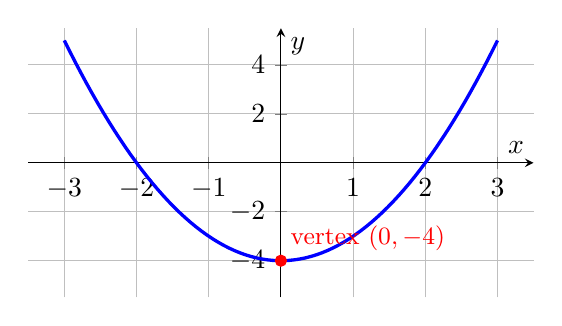
\begin{tikzpicture}
\begin{axis}[axis lines=middle,xlabel=$x$,ylabel=$y$,xmin=-3.5,xmax=3.5,ymin=-5.5,ymax=5.5,width=8cm,height=5cm,grid=both,xtick={-3,-2,-1,1,2,3},ytick={-4,-2,2,4},samples=80]
\addplot[very thick,blue,domain=-3:3]{x^2-4};
\addplot[only marks,mark=*,red] coordinates {(0,-4)};
\node[above right,red,font=\small] at (axis cs:0,-4) {vertex $(0,-4)$};
\end{axis}\end{tikzpicture}\end{center}
\vspace{0.2cm}\hrule\vspace{0.35cm}
\textbf{Directions: For each function state max or min, give the vertex, and the increasing / decreasing intervals.}

\begin{multicols}{2}
\begin{enumerate}[label=\textbf{\arabic*.}, start=1, itemsep=3cm]
  \item $\displaystyle y=x^{2}+2$
  \item $\displaystyle y=-x^{2}+5$
  \item $\displaystyle y=(x-3)^{2}$
  \item $\displaystyle y=-(x+1)^{2}-2$
  \item $\displaystyle y=(x+2)^{2}-1$
  \item $\displaystyle y=-(x-4)^{2}+3$
  \item $\displaystyle y=x^{2}-6x$
  \item $\displaystyle y=2(x-1)^{2}+3$
\end{enumerate}
\end{multicols}

\vspace{0.2cm}\hrule\vspace{0.3cm}
\textbf{Challenge} (same sheet):\\[4pt]
\begin{enumerate}[label=\textbf{\arabic*.}, start=9, itemsep=2.2cm]
  \item $y=(x-2)^{2}-9$ --- give the vertex, both intervals, and the two $x$-intercepts.
\end{enumerate}

\newpage

\begin{center}{\Large \textbf{Answer Key --- fully worked}}\end{center}
\vspace{0.25cm}
\textbf{Procedure:} Opens up ($+x^{2}$) gives a minimum; opens down gives a maximum; Vertex form $a(x-h)^{2}+k$ has vertex $(h,k)$; The graph turns (changes direction) at the vertex.\\[8pt]
\begin{enumerate}[label=\textbf{\arabic*.},itemsep=7pt]
  \item Opens up $\Rightarrow$ min; vertex $(0,2)$; dec $x<0$, inc $x>0$
  \item Opens down $\Rightarrow$ max; vertex $(0,5)$; inc $x<0$, dec $x>0$
  \item Vertex $(3,0)$, opens up $\Rightarrow$ min; dec $x<3$, inc $x>3$
  \item Vertex $(-1,-2)$, opens down $\Rightarrow$ max; inc $x<-1$, dec $x>-1$
  \item Vertex $(-2,-1)$, opens up $\Rightarrow$ min; dec $x<-2$, inc $x>-2$
  \item Vertex $(4,3)$, opens down $\Rightarrow$ max; inc $x<4$, dec $x>4$
  \item Complete the square: $x^{2}-6x=(x-3)^{2}-9$; vertex $(3,-9)$ min; dec $x<3$, inc $x>3$
  \item $a=2>0$ opens up $\Rightarrow$ min; vertex $(1,3)$; dec $x<1$, inc $x>1$
  \item Vertex $(2,-9)$ min; dec $x<2$, inc $x>2$; intercepts $x=-1,\ 5$
\end{enumerate}

\end{document}